\documentclass[%
	draft=true,
	paper=a4,%
	twoside=true,%
	abstract=true]{scrartcl}

\usepackage[utf8]{inputenc}
\usepackage[english]{babel}
\usepackage{microtype}
\usepackage{graphicx}
\usepackage[load-configurations=binary]{siunitx}
	\DeclareSIUnit\Molar{\textsc{m}}
\usepackage{svn-multi}
\usepackage{subfig}
\usepackage{booktabs}
\usepackage{fancyhdr}
\usepackage{tikz}
\usepackage{pgfplots}
\usepackage[numbers,square,sort&compress]{natbib}
\usepackage{scrtime}
\usepackage[version=3]{mhchem}
\usepackage{setspace}
	%\doublespacing
	%\onehalfspacing
\usepackage{lineno}
	\linenumbers\modulolinenumbers[2]
\usepackage{lastpage}	
\usepackage{xspace}
\usepackage[colorinlistoftodos,shadow]{todonotes}
\usepackage[autostyle]{csquotes}
\usepackage{listings}
\usepackage[backref]{hyperref}
 
% Subversion Information
\svnidlong
{$HeadURL$}
{$LastChangedDate$}
{$LastChangedRevision$}
{$LastChangedBy$}
\svnid{$Id$} 
 
\pagestyle{fancy}
\fancyfoot{}
\fancyfoot[OR]{\tiny Typeset on \today\ at \thistime\ from \href{\svnkw{HeadURL}}{SVN-Version \svnkw{LastChangedRevision}} | Page \thepage\ of \pageref{LastPage}}
\fancyfoot[EL]{\tiny Page \thepage\ of \pageref{LastPage} | Typeset on \today\ at \thistime\ from \href{\svnkw{HeadURL}}{SVN-Version \svnkw{LastChangedRevision}}}
 
\newcommand{\imsize}{\linewidth}
\newlength\imagewidth           % needed for scalebars
\newlength\imagescale           % ditto

\newcommand{\footremember}[2]{\footnote{#2}\newcounter{#1}\setcounter{#1}{\value{footnote}}}
\newcommand{\footrecall}[1]{\footnotemark[\value{#1}]}

\newcommand{\superscript}[1]{\ensuremath{^{\textrm{#1}}}}
\newcommand{\subscript}[1]{\ensuremath{_{\textrm{#1}}}}

\newcommand{\ie}{i.\,e.\xspace}
\newcommand{\Ie}{I.\,e.\xspace}
\newcommand{\eg}{e.\,g.\xspace}
\newcommand{\Eg}{E.\,g.\xspace}
\newcommand{\twod}{2\textsc{d}\xspace}
\newcommand{\threed}{3\textsc{d}\xspace}

\newcommand{\todomarco}[2][]{\todo[color=cyan!62!white,, #1]{Marco: #2}}
\newcommand{\todojcs}[2][]{\todo[color=magenta!62!white, #1]{Johannes: #2}}
\newcommand{\todome}[2][]{\todo[color=yellow!62!white, #1]{David: #2}}

\newcommand{\subfigureautorefname}{\figureautorefname} % make \autoref work with \subfloat
 
\title{Running Title: Acinar growth over lung development}
\subtitle{Typeset on \today\ at \thistime\ from Rev \svnkw{LastChangedRevision} (\svnday.\svnmonth.\svnyear\ \svnhour:\svnminute)}

\author{%
	David Haberthür\footremember{ana}{Institute of Anatomy, University of Bern, Switzerland}%
	\and Sébastien Barré\footrecall{ana}%
	\and Lilian Salm\footrecall{ana}%
	\and Marco Stampanoni\footremember{psi}{Swiss Light Source, Paul Scherrer Institut, Villigen, Switzerland}\ \footremember{eth}{Institute for Biomedical Engineering, Swiss Federal Institute of Technology and University of Zürich, Switzerland}%
	\and Johannes C. Schittny\footrecall{ana}%
	}
\date{}

\begin{document}
\renewcommand{\subsectionautorefname}{\sectionautorefname}
\renewcommand{\subsubsectionautorefname}{\sectionautorefname}
\maketitle

\begin{abstract}
Here be the Abstract\ldots
\end{abstract}
\listoftodos
\clearpage

\section{Introduction}\label{sec:Introduction}
Due a restricted availability of high resolution three-dimensional (\threed) imaging methods the knowledge about the development of the functional unit of the lung is limited. These functional units of the lung parenchyma are the so called pulmonary acini, which correspond to the gas-exchange volume in the lung which is ventilated by one purely conducting airway~\cite{Rodriguez1987}, see \autoref{fig:acinus schematic}.

Using synchrotron radiation based tomographic microscopy \cite{Haberthuer2010a} we developed a method to evaluate the volume of single acini throughout postnatal lung development.

\begin{itemize}
	\item adult rat at day 60 as example
	\item Volume of the functional lung units only determinable through \threed analysis including extraction of single acini
	\item Alveolar number counting with STEPanizer~\cite{Tschanz2011} $\rightarrow$ complete description of the functional units.
\end{itemize}

\renewcommand{\imsize}{.618\linewidth}
\begin{figure}
	\centering
	\pgfmathsetlength{\imagewidth}{\imsize}%
	\pgfmathsetlength{\imagescale}{\imagewidth/1635}%
	\def\x{1010}% scalebar-x at golden ratio of x=1635px
	\def\y{1831}% scalebar-y at 90% of height of y=2034px
	\def\shadow{10}% shadow parameter for scalebar
	\begin{tikzpicture}[x=\imagescale,y=-\imagescale]
		\clip (0,0) rectangle (1635,2034);
		\node[anchor=north west, inner sep=0pt, outer sep=0pt] at (0,0) {
\includegraphics[width=\imagewidth]{img/AcinusDiagram/Schittny2007a_edited.png}};
		\node at (810,75) [right] {Trachea};
		\node at (180,575) [right,rotate=28] {Pleura};
		\node at (325,650) [right] {Bronchi};
		\node at (515,1100) [left] {Bronchioli};
		\node at (700,1450) [left] {transitory Bronchioles};
		\node at (700,1700) [left] {Alveoli};
		\draw [|->,ultra thick] (1550,1329) -- (1550,400) node [midway,above,rotate=90] {Conducting Airways};
		\draw [|->,ultra thick] (1550,1349) -- (1550,1700) node [midway,above,rotate=90] {Gas-exchange}; % fill=white,semitransparent,text opacity=1
	\end{tikzpicture}%
	\caption{Schematic of the lung structure. The stages of one lung lobe are shown. On average rat lungs have ten generations of Bronchi and four generations of Bronchioli, which together form the conducting airways. The gas-exchanging region starts with one generation of transitory bronchioles which merge into alveolar ducts and end in the alveoli. Figure adapted from \cite{Schittny2007a}.}
	\label{fig:acinus schematic}%
	\todo[inline,caption={Copyright release?}]{How do we get a copyright release for this figure? How many generations of alveolar ducts are there in the rat? Just one?}
\end{figure}

The lung structure can be assessed using stereology~\cite{Hsia2010}, as shown by \citet{Tschanz2002}. Such an analysis is generally based on serial sections of the sample, thus the extracted information is a two-dimensional description \blockquote[\cite{Tschanz2002}]{of the parenchymal air space geometry and, due to geometric laws, it is not allowed to extrapolate these \twod statements directly to \threed structures}. With stereological methods it is fairly easy to extract global volume information\todojcs{From a region, from a ROI?}, but it not easily possible to extract such information from a functional unit of any organ, since it cannot easily be judged which detail on the microscopy slide belong to which functional unit in the three-dimensional compound.

\section{Materials \& Methods}\label{sec:MM}
\subsection{Rat lung samples}
Adult rat lung, day 60. Prepared according to \cite{Tschanz2002,Luyet2002}\todojcs{Which Publication should cite?}.

Briefly recapitulated, lung of 60 days old Sprague-Dawley rats were instilled with \SI{2.5}{\percent} glutaraldehyde (\cf{CH2(CH2CHO)2}) in \SI{0.03}{\Molar} potassium-phosphate buffer (pH 7.4) at a constant pressure of \SI{20}{\centi\meter} water column. At this applied pressure, the rat lung reaches its mid-respiratory volume. The instillation was performed via tracheotomy after opening the chest cavity and severing the diaphragm. After instillation and removal of the lung from the chest cavity, the instillation pressure was maintained during fixation (in the same fixative at \SI{4}{\celsius} for at least \SI{24}{\hour}) in order to prevent a recoiling of the lung.

After fixation, the samples were prepared for tomographic imaging, by postfixation with \SI{1}{\percent} osmium tetroxide (\cf{OsO4}) and staining with \SI{4}{\percent} uranyl nitrate (\cf{UO2(NO3)2}) to increase the x-ray absorption contrast. Using Histoclear (Merck KGaA, Darmstadt, Germany) as an intermedium the samples were then dehydrated in a graded series of ethanol and embedded in paraffin prior to mounting them onto standard scanning electron microscopy sample holders (PLANO GmbH, Wetzlar, Germany) also using paraffin~\cite{Tsuda2008}.

\subsection{Tomographic data acquisition}\label{sec:tomcat}
The tomographic experiments were performed at the \href{http://www.psi.ch/sls/tomcat/}{TOMCAT beamline} at the \href{http://www.psi.ch/sls/}{Swiss Light Source}, \href{http://www.psi.ch/}{Paul Scherrer Institut}, Villigen, Switzerland~\cite{Stampanoni2006a}. The samples were scanned at \SI{20.0}{\kilo\electronvolt}. After penetration through the sample, the x-rays were converted into visible light by a \SI{20}{\micro\meter} thick LuAG:Ce scintillator (Lutetium Aluminum Garnet activated by cerium, \cf{Lu3Al5O12}, from \href{http://www.crytur.cz/}{Crytur Ltd.}, Turnov, Czech Republic).

A 10\(\times\) magnifying, diffraction limited microscope optics was used to magnify the image on the \SI{18}{\micro\meter} thick Cerium doped Yttrium Aluminium Garnet (YAG) (\cf{Y3Al5O12}) scintillator screen. Subsequently, a high-resolution 2048\(\times\)2048 pixel CCD camera (\href{http://www.pco.de/sensitive-cameras/pco2000/}{pco.2000}, \href{http://www.pco.de/}{PCO AG}, Kelheim, Germany) with \SI{14}{\bit} dynamic range was used to digitize this magnified image. To reduce imaging noise and increase the acquisition speed, we operated the detector in 2\(\times\)2 binning mode. As a result, the pixel size was \SI{1.48}{\micro\meter} and the exposure time was between \SIrange{160}{180}{\milli\second}. The details of the beamline setup have been described by \citet{Stampanoni2006a}.

To be able to safely distinguish the alveolar septa (approx.~\SIrange{3}{8}{\micro\meter} thick\todojcs{Correct?}) the tomographic images used for analysis of the functional units of the lung need to have a resolution in the order of one to two microns. Since we selectively wanted to extract a large amount of single acini\todo[caption={How many acini are there?}]{Do we have data on how many and how large acini there are in the rat lung? $\rightarrow$ Sébastien}, we not only needed to acquire high resolution tomographic scans, but a acquire a dataset with both large volume and very high resolution. Usually---with classic microscopy based imaging methods---a large field of view can only be acquired with low magnification and vice-versa. Thus, the full volume of our samples would not have fit inside the classic field of view of the TOMCAT beamline at the aforementioned optical properties (1.52\(\times\)1.52\(\times\)\SI{1.52}{\milli\meter}). To overcome this problem, we enhanced the enhance the field of view of the TOMCAT beamline at the chosen optical configuration. This enhancement was done with the so called wide-field scanning protocol, described prior by \citet{Haberthuer2010}.

Briefly summarized, the wide-field scanning process merges several independently acquired partial tomographic scans which altogether cover the desired field of view. After acquisition, single projections of the partial scans are merged to one large projection spanning the desired field of view. The merging of the single projections was implemented on the tomographic reconstruction cluster of seven \SI{64}{\bit} Opteron machines with four cores and \SI{8}{\giga\byte} RAM each. This implementation on the cluster made it possible to use the classic tomographic reconstruction workflow at TOMCAT, which has been described in detail by \citet{Hintermueller2010}.

With this approach we increased the lateral field of view at TOMCAT three-fold, while keeping both voxel size and reconstruction quality on the desired level and avoiding the aforementioned trade-off between voxel size and sample volume. Since we also performed a so called stacked scan in relation to the z-axis of the tomographic setup, we even further increased the field of view and recorded volume of our samples. Finally, we acquired tomographic dataset of approximately 3000\(\times\)3000\(\times\)3072 pixels with \SI{1.48}{\micro\meter} pixel size. This corresponds to a 9-fold increase in recorded volume as compared to one classic scan at TOMCAT, giving us the advantage of both high resolution images and large visible sample volume.

\subsection{Visualization and Extraction of Acini}
The tomographic datasets of the sample were three-dimensionally analyzed and visualized using \href{http://mevislab.de}{MeVisLab} (Version 2.1 (2010-07-26 Release)~\cite{Bitter2007}, MeVis Medical Solutions AG and Fraunhofer MEVIS - Institute for Medical Image Computing, Bremen, Germany). The calculations have been performed on a Dell Precision T7500 work station (\SI{24}{\giga\byte} RAM, Intel Xeon CPU X5550 at \SI{2.66}{\giga\hertz}, Windows 7 Professional \SI{64}{\bit}).

\subsubsection{Preprocessing}
The tomographic datasets obtained at TOMCAT were converted from a stack of TIFF-files to the native GVR format of MeVisLab, a multi-resolution \href{https://secure.wikimedia.org/wikipedia/en/w/index.php?title=Octree&oldid=409131920}{octree}-based image format. This permitted us to easily switch between resolutions in the dataset to interactively perform the visualization and analysis on a lower resolution prior to the final analysis on full resolution datasets.

\subsubsection{Manhole Covers}\label{sec:manhole covers}
On binned datasets we extracted conducting airway segments (see \autoref{fig:acinus schematic}) using a threshold interval based region growing algorithm~\cite{Zucker1976}. A seed point for the region growing algorithm was manually defined inside the terminal bronchiole or alveolar duct on one of the most proximal slices of the dataset (shown in \autoref{subfig:sample}). This approach made it possible to extract a connected airway segment, which was then further divided in conducting and gas-exchanging airways. This division was performed with manually placed circular segmentations stoppers, which we dubbed manhole covers (shown as red discs in \autoref{subfig:airway segment} and \subref*{subfig:extracted acini}). The manhole covers were manually placed in the airway segment based on morphological criteria, \ie on changes in the airway wall structure which mark the entrance point into the acinus.

\renewcommand{\imsize}{\linewidth}
\begin{figure}
	\centering
	\pgfmathsetlength{\imagewidth}{\imsize}%
	\pgfmathsetlength{\imagescale}{\imagewidth/1740}%
	\def\x{1075}% scalebar-x at golden ratio of x=1740px
	\def\y{894}% scalebar-y at 90% of height of y=993px
	\def\shadow{11}% shadow parameter for scalebar
	\begin{tikzpicture}[x=\imagescale,y=-\imagescale]
		\clip (0,0) rectangle (1740,993);
		\node[anchor=north west, inner sep=0pt, outer sep=0pt] at (0,0) {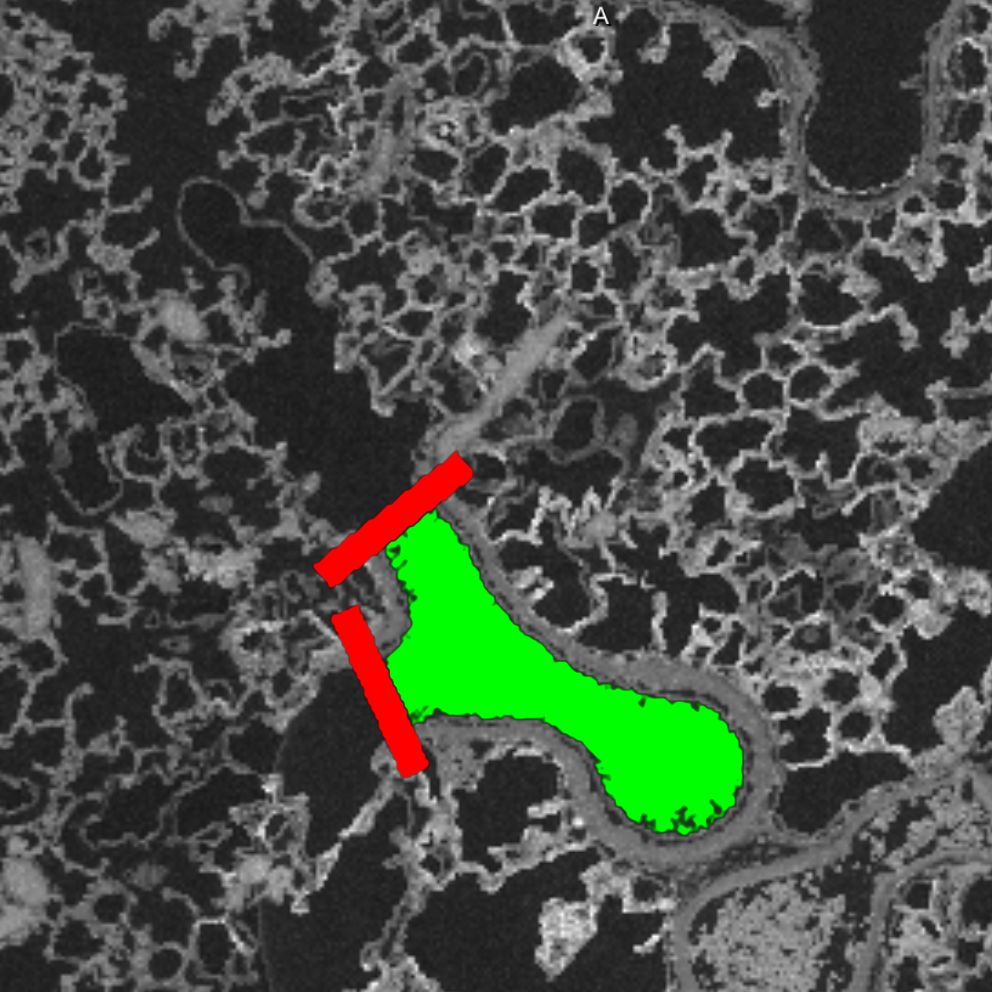
\includegraphics[width=\imagewidth]{img/ManholeCoverExplanation/SliceSomeWhereAtTheBottom}};
		% 492px = 0.8mm > 100px = 163um > 308px = 500um, 62px = 100um
		\draw[|-|,blue,thick] (1728,250) -- (1728,742) node [sloped,midway,below,fill=white,semitransparent,text opacity=1] {\SI{0.8}{\milli\meter} (800px) TEMPORARY!};
	\draw[|-|,thick] (\x+\shadow,\y+\shadow) -- (\x+308+\shadow,\y+\shadow) node [midway, above] {\SI{500}{\micro\meter}};
		\draw[|-|,white,thick] (\x,\y) -- (\x+308,\y) node [midway,above] {\SI{500}{\micro\meter}};
		\draw[yellow,dashed,thick] (584,422) circle (40);
		\draw[yellow,dashed,thick] (536,374) circle (40);
		\draw[yellow,dashed,thick] (493,506) circle (40);
		\draw[yellow,dashed,thick] (442,438) circle (40);						
	\end{tikzpicture}%
	\caption{Slice showing extracted conducting airway (green) and manhole cover (red). The dashed yellow circles highlight some examples of outpouchings of the airway wall which mark the change from conducting to gas-exchanging regions. Between these regions we semiautomaticall placed the manhole covers.}
	\label{fig:ManholeCoverExplanation}
\end{figure}

Using a separate region growing module, we subsequently extracted single acini from the datasets (shown as yellow volumes in \autoref{subfig:extracted acini}) automatically. The manhole covers\footnote{The manhole covers were implemented through a \href{http://www.mevis-research.de/cgi-bin/discus/board-auth.cgi?lm=1282233250&file=/839/11760.html}{custom module (\emph{XMarkerClipPlanes})} by Milo Hindennach, a member of the MeVis Developer team.} placed in the first step are fully defined through their diameter and \href{https://secure.wikimedia.org/wikipedia/en/w/index.php?title=Surface_normal&oldid=411684319}{surface normal}. This made it possible to automatically define the seed point for additional region growing modules used for the extraction of the single acini. We simply flipped the direction of the surface normal and placed the seed point along this vector slightly behind the manhole cover, inside the acinar airspace. The only manual work left was the iterative selection of the correct gray value threshold used for the region growing segmentation.

\renewcommand{\imsize}{.5\linewidth}
\pgfmathsetlength{\imagewidth}{\imsize}%
\pgfmathsetlength{\imagescale}{\imagewidth/1008}%
\def\x{50}% scalebar-x at golden ratio of x=1008px
\def\y{916}% scalebar-y at 90% of height of y=1018px
\begin{figure}
	\centering
	\subfloat[Sample]{%
		\begin{tikzpicture}[x=\imagescale,y=-\imagescale]
			\node[anchor=north west, inner sep=0pt, outer sep=0pt] at (0,0) {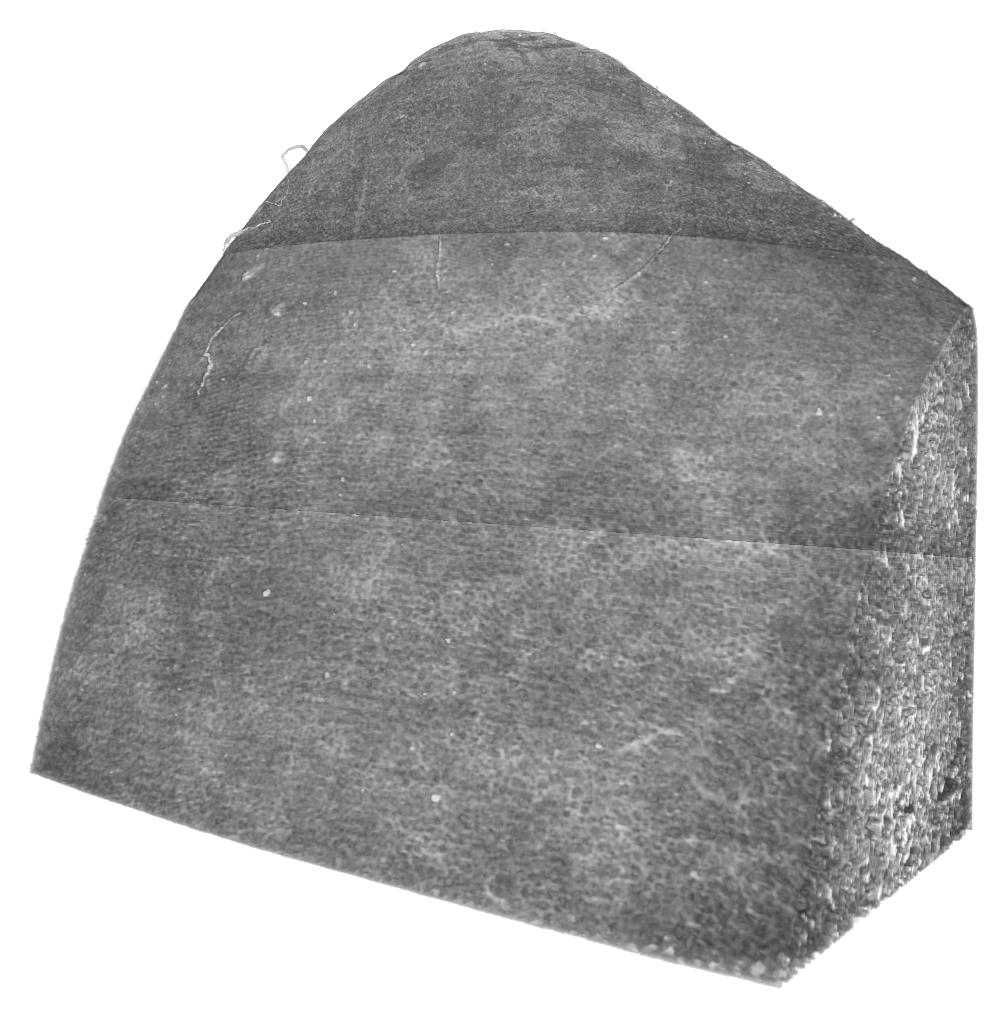
\includegraphics[width=\imagewidth]{img/ManholeCover/R108C60B_2010c_Acinus_Sample}};
			% 774px = 4.363mm > 100px = 564um > 89px = 500um, 18px = 100um
			\draw[|-|,blue,thick] (775,990) -- (33,771) node [sloped,midway,above,fill=white,semitransparent,text opacity=1] {\SI{4.363}{\milli\meter} (2948px) TEMPORARY!};
			\draw[|-|, thick] (\x,\y) -- (\x+89,\y) node [right] {\SI{500}{\micro\meter}};
		\end{tikzpicture}%
		\label{subfig:sample}%
		}
	\subfloat[Conducting airways with manhole covers]{%
		\begin{tikzpicture}[x=\imagescale,y=-\imagescale]
			\node[anchor=north west, inner sep=0pt, outer sep=0pt] at (0,0) {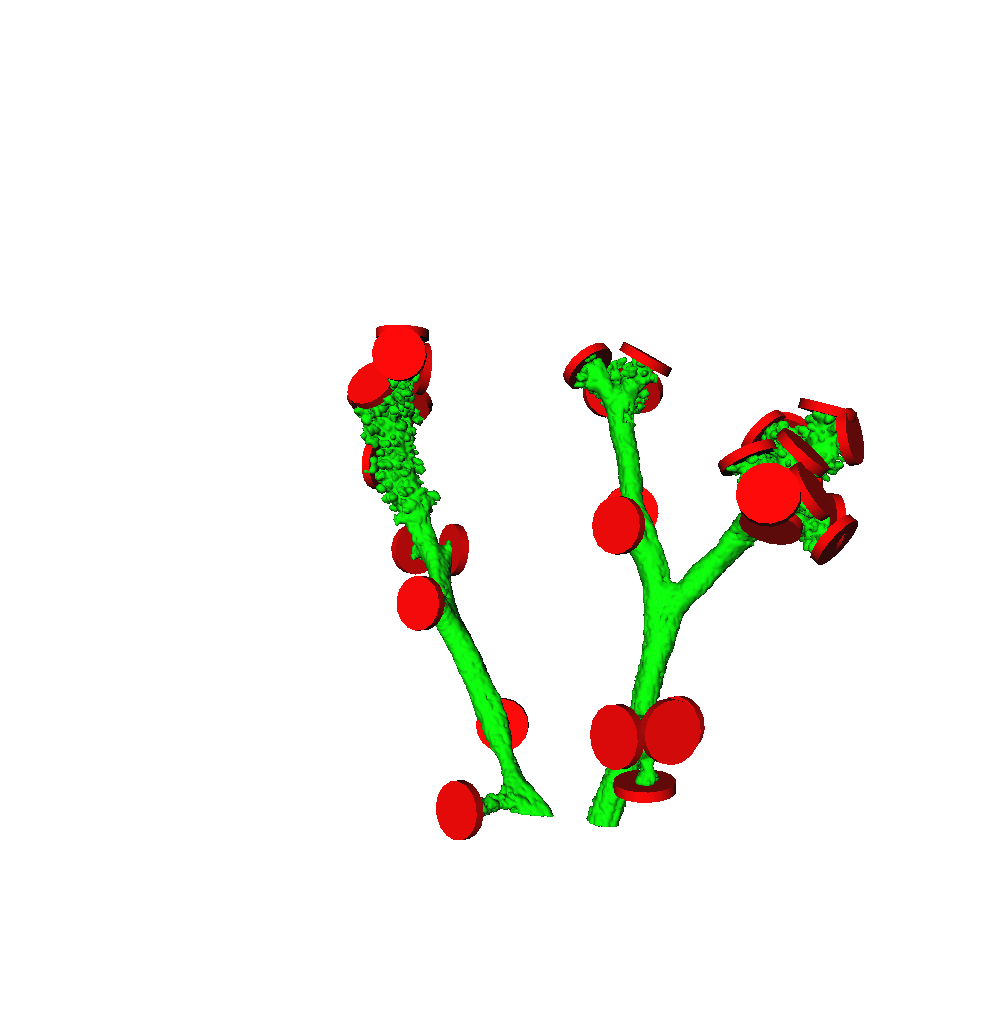
\includegraphics[width=\imagewidth]{img/ManholeCover/R108C60B_2010c_Acinus_Airspace}};
			\draw[|-|, thick] (\x+450,\y) -- (\x+89+450,\y) node [right] {\SI{500}{\micro\meter}};
		\end{tikzpicture}%
		\label{subfig:airway segment}%
		}\\
	\subfloat[Several extracted acini. Semitransparent Sample.]{%
		\begin{tikzpicture}[x=\imagescale,y=-\imagescale]
			\node[anchor=north west, inner sep=0pt, outer sep=0pt] at (0,0) {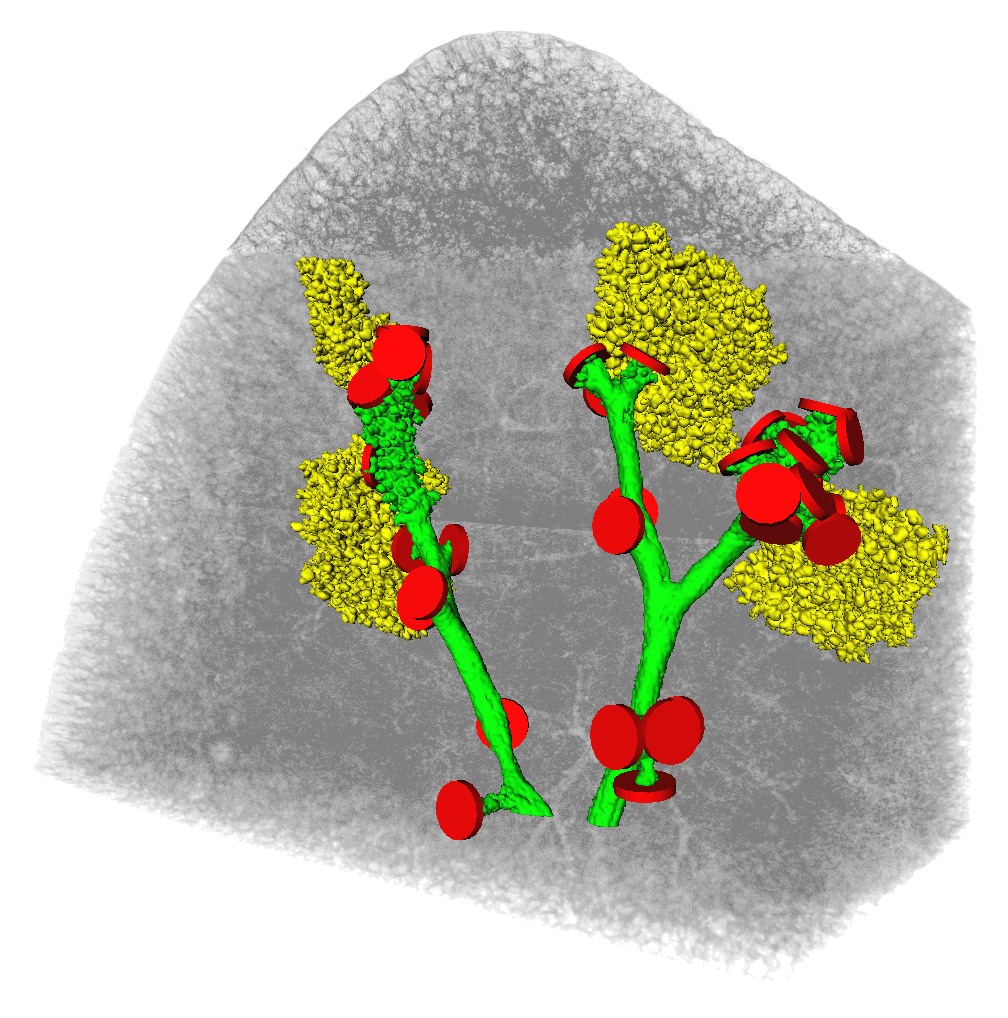
\includegraphics[width=\imagewidth]{img/ManholeCover/R108C60B_2010c_Acinus_Overlay}};
			\draw[|-|, thick] (\x,\y) -- (\x+89,\y) node [right] {\SI{500}{\micro\meter}};
		\end{tikzpicture}%
		\label{subfig:extracted acini}%
		}
	\subfloat[Several extracted acini. Non-transparent Sample.]{%
		\begin{tikzpicture}[x=\imagescale,y=-\imagescale]
			\node[anchor=north west, inner sep=0pt, outer sep=0pt] at (0,0) {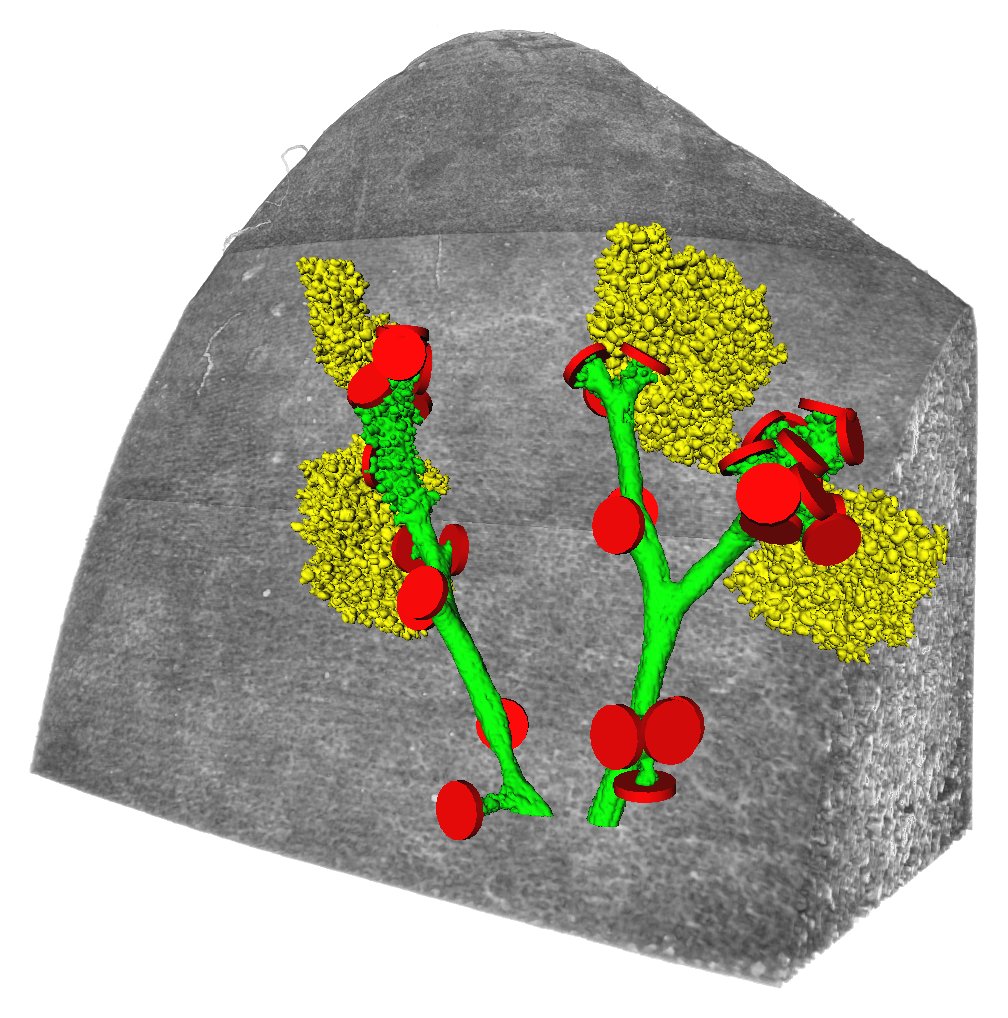
\includegraphics[width=\imagewidth]{img/ManholeCover/R108C60B_2010c_Acinus_OverlayNonTransparent}};
			% 774px = 4.363mm > 100px = 564um > 89px = 500um, 18px = 100um
			\draw[|-|, thick] (\x,\y) -- (\x+89,\y) node [right] {\SI{500}{\micro\meter}};
		\end{tikzpicture}%
		\label{subfig:extracted acini2}%
		}
	\caption{Visualization of the work flow for the extraction of the acinar volumes: %
		\subref{subfig:sample}: \threed visualization of sample. For this sample, we stacked three wide-field scans on top of each other, increasing the field of view nine-fold compared to a classic scan at TOMCAT. %
		\subref{subfig:airway segment} Extracted airway segment (green). Using a threshold based region growing algorithm, we extracted conducting airways inside the sample. The red discs shown are the so-called manhole covers, which were used as segmentation stoppers for the region growing. %
		\subref{subfig:extracted acini} Extracted acini (yellow). Several extracted acini are shown superimposed over the sample in \threed. For each such acinus we recorded the volume.%
		}
	\label{fig:workflow}
	\todo[inline]{Do we want to keep \autoref{subfig:extracted acini} or \ref{subfig:extracted acini2} (semitransparent or opaque sample)?}
\end{figure}

The volume of the single acini was calculated by multiplying the amount of segmented voxels with the voxel volume, tabulated in several Excel-Files and prepared for analysis. The segmented acini were also exported to single \href{https://secure.wikimedia.org/wikipedia/en/w/index.php?title=Digital_Imaging_and_Communications_in_Medicine&oldid=415023605}{DICOM} stacks to facilitate further processing in either MeVisLab, \href{http://rsbweb.nih.gov/ij/}{ImageJ}~\cite{Abramoff2004} or the \href{http://stepanizer.com/}{Stepanizer}~\cite{Tschanz2011}, as defined later on.

\begin{itemize}
	\item Overlay of acini with Original dataset to use them in STEPanizer
\end{itemize}

\section{Stereological Analysis}
\begin{itemize}
	\item Quick rundown on Stereology, including “how to do it correctly”/ATS guidelines by \citet{Hsia2010}.
	\item STEPanizer; web based tool, counting with line pairs and automatic tabulation in Excel-Files.
	\item Analysis for Volume and Surface, comparison of MeVisLab and STEPanizer-data.
\end{itemize}

\section{Results}\label{sec:Results}
For each day and sample we extracted multiple \todome{how many exactly?} acini with the Manhole Cover-method described in \autoref{sec:manhole covers}. A summary of the data from the extracted acinar volumes is shown in \autoref{tab:summary}. The data has been analyzed using R (Version 2.12.1 (2010-12-16)~\cite{R} in RStudio (\url{http://rstudio.org/}, Version 0.94.84). 

% FROM R
%summary(TotalVolumes)
%       V1                  V2                  V3                  V4                  V5           
% Min.   :4.934e-04   Min.   :1.330e-03   Min.   :1.520e-04   Min.   :2.442e-03   Min.   :2.039e-03  
% 1st Qu.:4.100e-03   1st Qu.:6.502e-03   1st Qu.:1.192e-02   1st Qu.:3.892e-02   1st Qu.:2.742e-02  
% Median :8.597e-03   Median :1.124e-02   Median :2.951e-02   Median :6.950e-02   Median :5.259e-02  
% Mean   :1.178e-02   Mean   :1.398e-02   Mean   :3.707e-02   Mean   :8.069e-02   Mean   :6.472e-02  
% 3rd Qu.:1.805e-02   3rd Qu.:1.977e-02   3rd Qu.:5.588e-02   3rd Qu.:1.099e-01   3rd Qu.:1.014e-01  
% Max.   :3.908e-02   Max.   :3.855e-02   Max.   :1.202e-01   Max.   :2.109e-01   Max.   :1.907e-01  
% NA's   :7.980e+02   NA's   :7.820e+02   NA's   :7.790e+02   NA's   :7.990e+02   NA's   :8.440e+02  
 
\begin{table}
	\centering
	\caption{Summary of the extracted Data. All volumes are given in \si{\micro\litre}}
	\noindent\makebox[\textwidth]{%
	\begin{tabular}{rccccc}
		\toprule
		& Day 04 & Day 10 & Day 21 & Day 36 & Day 60\\
		\midrule
		& Data \\
		\bottomrule
	\end{tabular}
	}
	\label{tab:summary}
	\todo[inline]{from “summary(TotalVolumes)” in R-Studio}
\end{table}

\begin{itemize}
	\item Show volumes of different acini with MeVisLab and STEPanizer
	\item What about shrinkage?
	\item Comparison with other data?
	\item What about the surface? What about the “Erithrocytes”?
	\item Alveolar number, how can we bring in this data?
\end{itemize}

\section{Discussion}\label{sec:Discussion}
We hypothesize that this large increase of the acinar volume can only be achieved by a conversion of the \numrange{2}{4} most distal purely conducting airways into alveolar ducts between birth and adulthood. As a consequence \numrange{4}{16} small acini have to be merged to a larger one. We expect that the increased complexity of the adult acini influences both ventilation and particle deposition.

\section{Contributions}
\begin{itemize}
	\item David Haberthür helped with rat lung sample extraction, data acquisition and analysis of the acinar volume, creation of the MeVisLab networks for extraction of the acini, analysis of the data in the STEPanizer statistical analysis and main writer of the manuscript.
	\item Sébastien Barré was helping with preparations of the samples, data acquisition,  preprocessing and analysis of the datasets.
	\item Lilian Salm: Alveolar numbers
	\item Marco Stampanoni: TOMCAT
	\item Johannes C. Schittny: Group head, grant writer and lung extractor.
\end{itemize}

\section{Acknowledgments}
We thank Federica Marone, Beamline Scientist at TOMCAT for the long-standing great support at the Beamline and implementation of the reconstruction of the merged wide-field scanning projections on the TOMCAT cluster. Christoph Hinterm\"{u}ller, former member of the TOMCAT group, and now Project Management \& Research at \href{http://gtec.at/}{g.tec medical engineering GmbH} also helped us during countless shifts at the beamline. He also helped with the first implementation of wide-field scanning at TOMCAT. Bernd Pinzer, Post-Doc at TOMCAT adopted the support of our group from Chris and also does great job. Milo Hindennach, MeVis Developer at Fraunhofer MEVIS provided the \href{http://www.mevis-research.de/cgi-bin/discus/board-auth.cgi?lm=1282233250&file=/839/11760.html}{Manhole cover module in MeVisLab}, which is still at the core of the MeVisLab-network used in this publication. We thank Mohammed Ouanella, our former lab technician, for expert technical assistance in the lab\todo{Eveline?}.

The handling of animals before and during the experiments, as well as the experiments themselves, were approved and supervised by the Swiss Agency for the Environment, Forests and Landscape and the Veterinary Service of the Canton of Bern, Switzerland.

This work has been funded by the grants 3100A0-109874 and 310030-125397 \todo{Still correct?} of the Swiss National Science Foundation.

\bibliographystyle{unsrtnat}
\bibliography{../references}

\appendix
\section{Listings}
Do we provide code-listings for \href{http://reproducibleresearch.net}{reproducible research}?
\subsection{R}
\verb+p:\doc\#R\AcinusPaper\AcinarPlot.r+: Script to analyze the extracted acinar volume data and to generate \autoref{fig:boxplot}.

\subsection{MeVisLab}
\begin{itemize}
	\item \href{http://www.mevis-research.de/cgi-bin/discus/board-auth.cgi?lm=1282233250&file=/839/11760.html}{XMarkerClipPlanes}: Custom MeVisLab-Module by Milo Hindennach, used to define the manhole covers in \threed at the borders between conducting and gas-exchanging regions in the extracted airspace.
	\item One example file from \verb+p:\doc\MeVisLab-Networks\2010\AcinarTreeExtraction\+? Or at least one associated GUI-Script? Or can/should we grant access to \href{http://code.ana.unibe.ch/websvn/listing.php?repname=MeVisLab-Networks}{my MeVisLab SVN-repo}? I’d do it!
\end{itemize}
 
\end{document}